
\subsection{RoboCup}

\begin{frame}{La compétition RoboCup (1/2) -- Origine et ambition}
    \begin{columns}
        \begin{column}{0.45\linewidth}
            \begin{block}{RoboCup}
                Compétition internationale
            \end{block}
            \begin{block}{Ambition -- 2050}
                Battre la meilleure équipe humaine de football
            \end{block}
            \vspace{1.0em}
            \begin{itemize}
                \setlength\itemsep{1.0em}
                \item Origine (1997) : victoire
                    aux échecs contre Garry Kasparov
                \item $\Rightarrow$ Grand défi pour l'IA
            \end{itemize}
        \end{column}
        \begin{column}{0.55\linewidth}
            \centering
            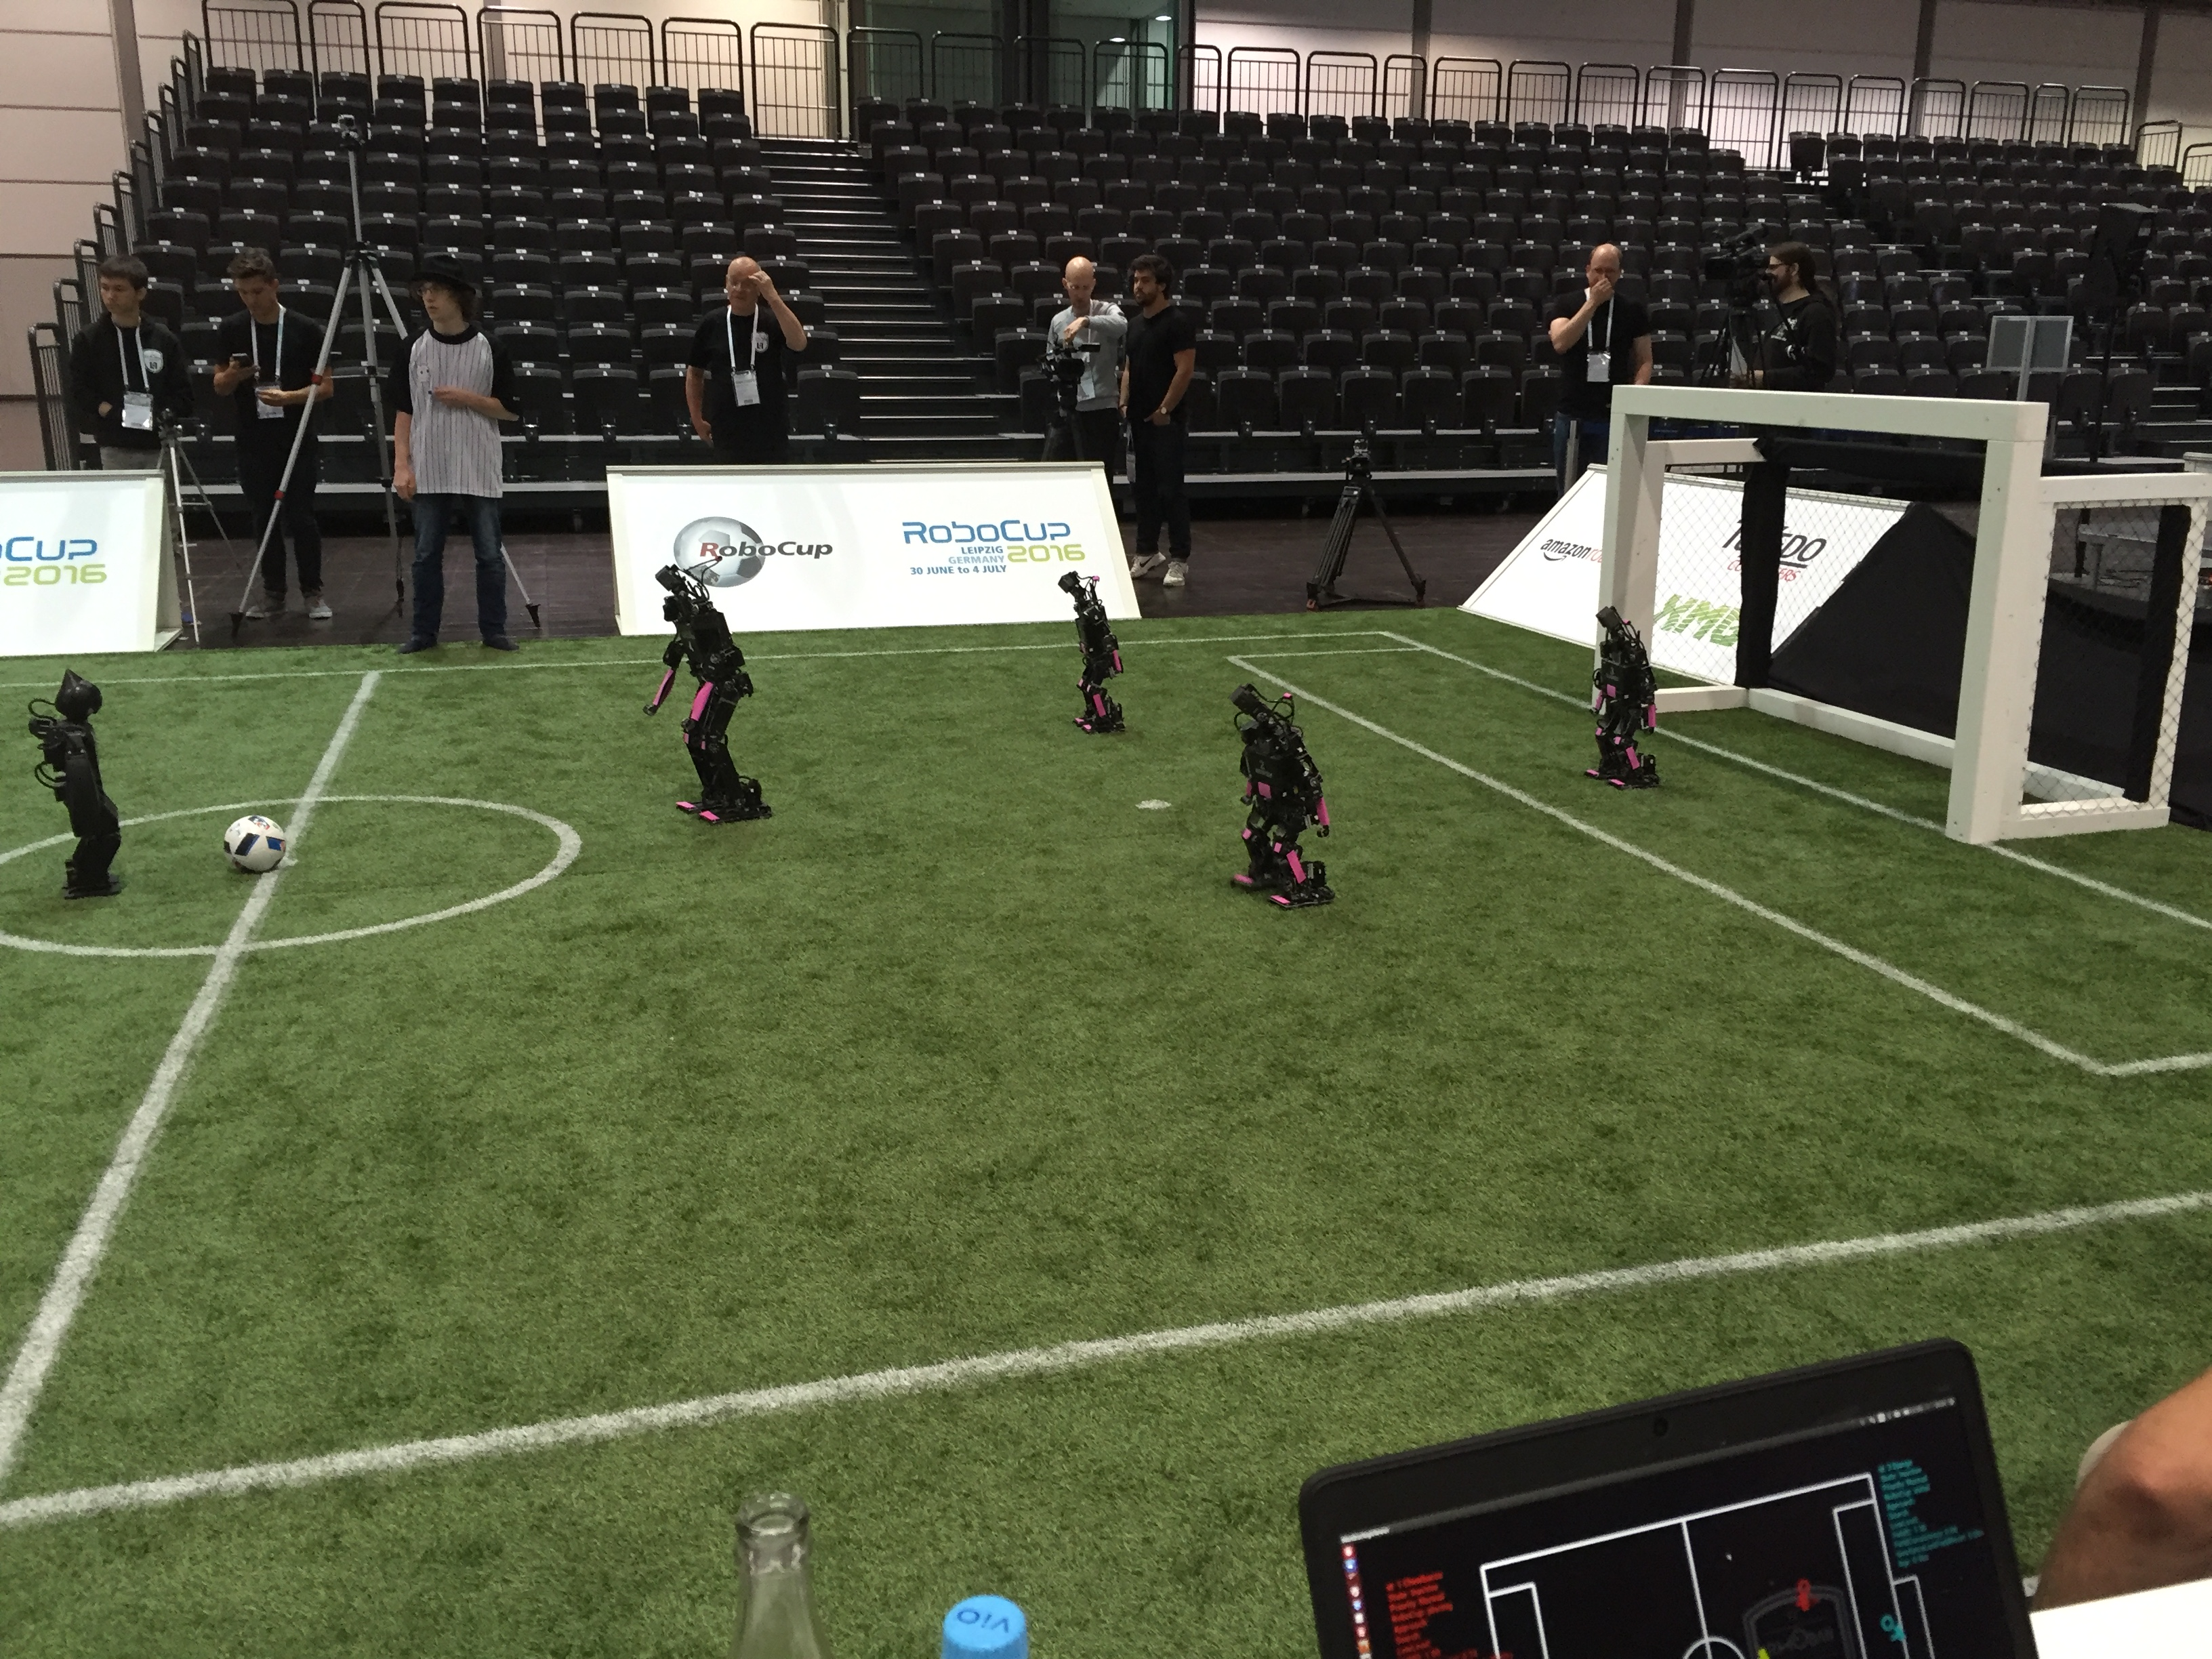
\includegraphics[width=1.0\linewidth]{../media/robocup_field.jpg}
        \end{column}
    \end{columns}
\end{frame}

\begin{frame}{La compétition RoboCup (2/2) -- Ligue \textit{Humanoid}}
    \begin{columns}
        \begin{column}{0.45\linewidth}
            3 tailles : 
            \textit{Kid-Size}, \textit{Teen-Size}, \textit{Adult-Size}\\
            \vspace{1.0em}
            \begin{block}{Ligue \textit{Humanoid Kid-Size}}
                Robots autonomes, anthropomorphe et non standards
            \end{block}
            \begin{itemize}
                \item Recherche : 
                    mécatronique, mouvements, perception
                \item Contraintes opérationnelles
            \end{itemize}
            \vspace{1.0em}
            \textit{Rhoban Football Club} : 
            1ère place \textit{Humanoid Kid-Size} en 2016 et 2017\\
        \end{column}
        \begin{column}{0.55\linewidth}
            \centering
            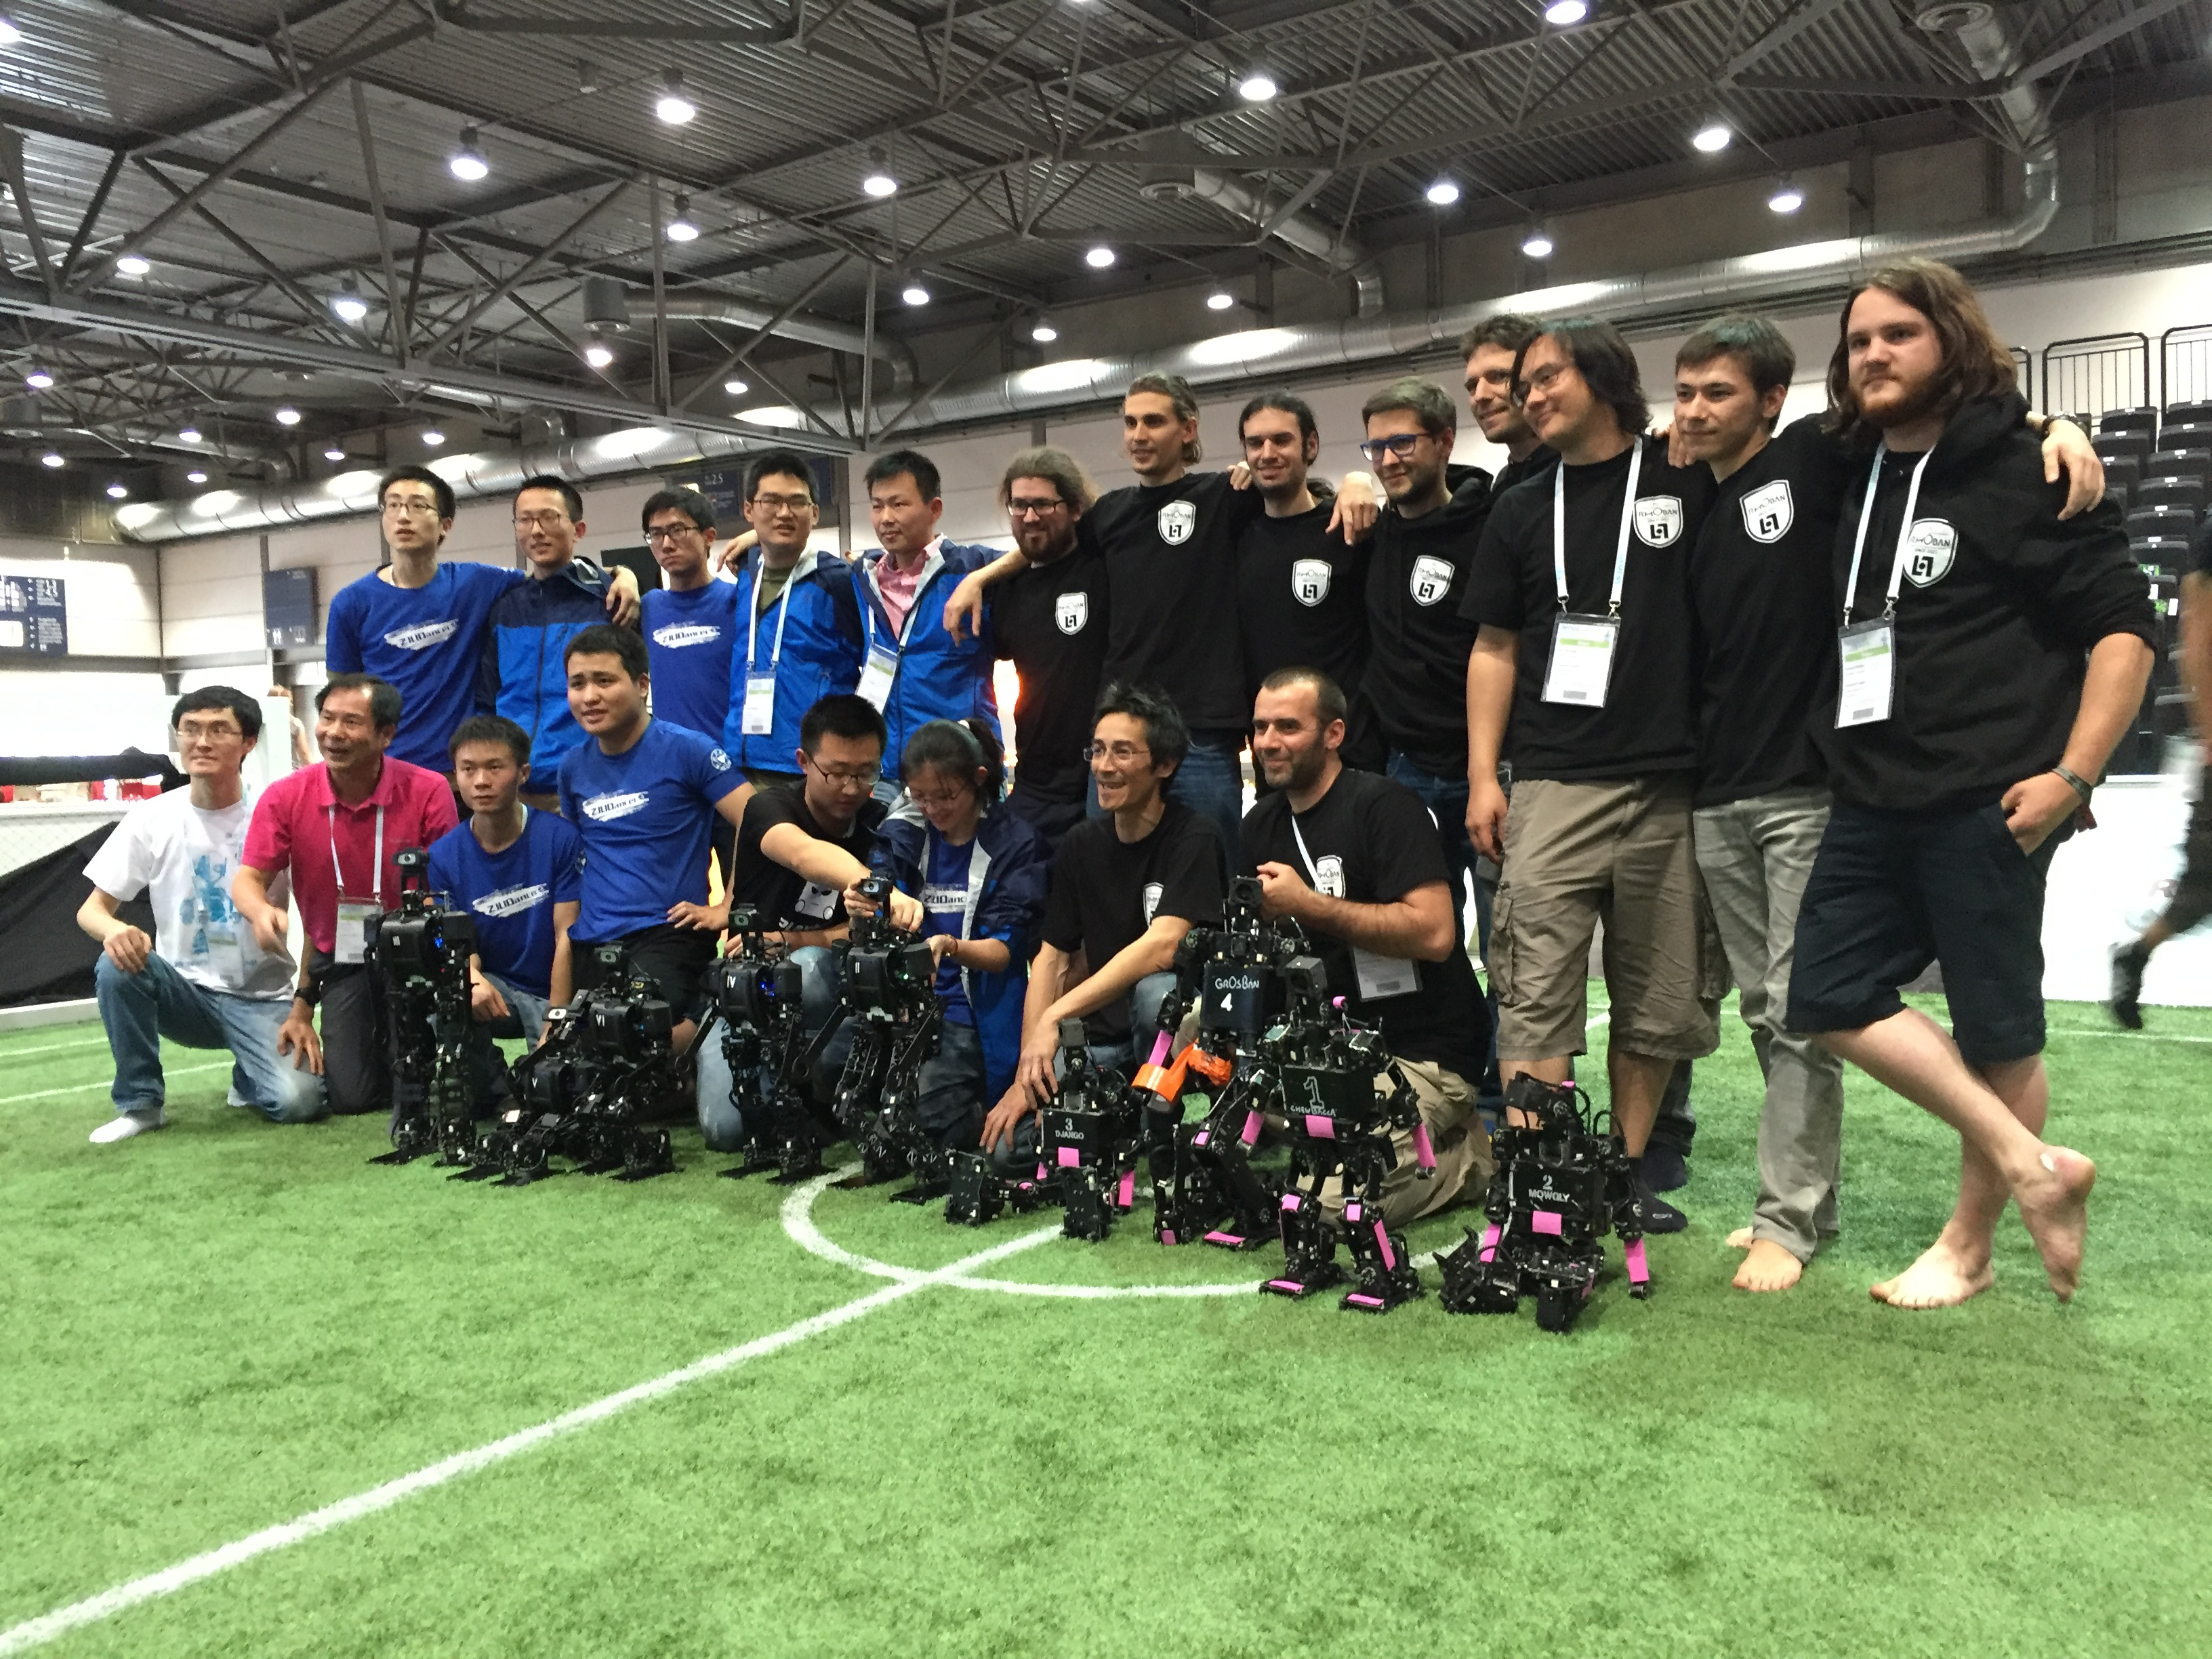
\includegraphics[width=1.0\linewidth]{../media/robocup_team.jpg}
        \end{column}
    \end{columns}
    \begin{block}{}
        \customtextcolor{
            \small
            \textit{Rhoban football club: Robocup humanoid kid-size 2016 champion team paper}}\\
        \scriptsize
        Julien Allali, Louis Deguillaume, Rémi Fabre, Loic Gondry, Ludovic Hofer, Olivier Ly, 
        Steve N'Guyen, Grégoire Passault, Antoine Pirrone, Quentin Rouxel\\
        RoboCup 2016\\
    \end{block}
\end{frame}
